\documentclass[a4paper]{article}
\setlength{\headheight}{1.1\baselineskip}
%\usepackage[margin=1.0 in]{geometry}
%\renewcommand{\baselinestretch}{1.5}

\usepackage[english]{babel}
\usepackage[utf8]{inputenc}
% package for including graphics with figure-environment
\usepackage{graphicx}
\usepackage{hyperref}
% colors for hyperlinks
% colored borders (false) colored text (true)
\hypersetup{colorlinks=true,citecolor=black,filecolor=black,linkcolor=black,urlcolor=black}

% package for bibliography
%\usepackage[authoryear,round]{natbib}
% package for expectation signs
\usepackage{amsmath,amssymb,mathtools,bm,etoolbox}
%\documentclass[a4paper,11pt]{report} 
\usepackage{breqn}
\usepackage{amsmath}
\usepackage{enumitem} 
\usepackage{amsmath, amsthm, amssymb}
\usepackage{amsmath}
\newcommand{\abs}[1]{ \left\lvert#1\right\rvert} 
\newcommand{\norm}[1]{\left\lVert#1\right\rVert}
% package for header
\usepackage[automark]{scrpage2}
\pagestyle{scrheadings}
\ihead[]{Isa Marques, Xi Sun, Xueying Liu}
\ohead[]{\today}
\cfoot[]{\pagemark} 
\setheadsepline[122mm]{0.3mm}
\usepackage{csquotes}



% some more packages enabling table and figure production
\usepackage{float, afterpage, rotating, graphicx}
\usepackage{epstopdf}
\usepackage{longtable, booktabs, tabularx}
\usepackage{fancyvrb, moreverb, relsize}
\usepackage{eurosym, calc, chngcntr}
\usepackage{caption}
\usepackage{mdwlist}
\usepackage{xfrac}
\usepackage{setspace}
\usepackage{xcolor}
\usepackage{multirow}
%\usepackage{booktabs}


% packages for bibliography
\usepackage[backend=biber, natbib=true,style=numeric]{biblatex}
\AtBeginDocument{\toggletrue{blx@useprefix}}
\AtBeginBibliography{\togglefalse{blx@useprefix}}
\setlength{\bibitemsep}{1.5ex}
\addbibresource{refs.bib}




\begin{document}
	\title{
	%\begin{figure}[!ht]
	%	\flushleft
	%		\includegraphics[width=0.7\textwidth]{logo.eps}
	%\end{figure}
	\vspace{1cm}
	\Huge \textbf{ Semiparametric Single Index Models }\\ \Large Ichimura's and Klein and Spady's methods \\
	}
	
	\vspace{1cm}
	
	% if you are the only author, you might use the following
	% \author{Name of student}	
	
	% Insert here your name and correct mail address
	\author{\Large \href{mailto:first.student@smail.fh-koeln.de}{Isa Marques}\and \Large \href{mailto:second.student@smail.fh-koeln.de}{Xi Sun} \and \Large \href{mailto:second.student@smail.fh-koeln.de}{Xueying Liu}
	\vspace{1cm}}
	
	% name of the course and module
	\date{
	\large University of Bonn \\ Project Module in Econometrics and Statistics\\ 
	\vspace{0.8cm}
	\large Prof. Dr. Kneip \\
	\large Prof. Dr. Liebl \\
	\vspace{1cm}
	\today
	}

	\maketitle
	\setlength{\parindent}{0pt}

\vspace{2cm}
\begin{abstract}

Semiparametric single index models are widely applied in economic research. Applications range from finance to labor economics. This paper focuses on Ichimura's (1993) and Klein and Spady's (1993) models. These models help us dig into the vast field of semiparametric single index regression models, while still leaving much behind. In particular, both of these models are based on iterative optimization methods, which are in general computationally costly. The structure of the paper consists of three blocks of analysis: theoretical outline; monte carlo simulations; and a real data set example, using the pre-processed Gender Recognition by Voice and Speech Analysis dataset.

\end{abstract}
%	\newpage
%	\tableofcontents
	\newpage
	
\section{Introduction} % (fold)
\label{sec:introduction}

Semiparametric single index models are widely applied in economic research. Applications range from finance to labor economics. Masten and Masten (2015) \cite{[30]} use Klein and Spady's (1993) \cite{[12]} semiparametric single index model to predict bankruptcies, as opposed to the logit model, the standard parametric model for bankruptcy prediction. Coelho et al. (2005) \cite{[29]} use the same semiparametric single index model to analyze female labor market in Portugal. Moreover, McMillen and Thorsnes (2012) \cite{[31]} adopt a semiparametric single index average derivative estimator to study the effect of copper smelter on house prices in Tacoma.

This paper focuses on Ichimura's (1993) \cite{[6]} and Klein and Spady's (1993) \cite{[12]} models. These models help us dig into the vast field of semiparametric single index regression models, while still leaving much behind. In particular, both of these models are based on iterative optimization methods, which are in general computationally costly. A natural attraction of Klein and Spady's (1993) \citep{[12]} model is the fact that it reaches the semiparametric efficiency bound. Thus, in that sense, one can say it is fully efficient  (Cameron and Trivedi, 2005 \cite{[5]}). However, it is at fault comparatively to Ichimura's (1993) \cite{[6]} due to its lack of generality, as it is restricted to the binary case.

The structure of the paper consists of three blocks of analysis: theoretical outline; simulations, where small sample properties are analyzed; and a real data set example, where one can illustrate the behavior of the models on an applied framework. All parties contributed to the presentation and the writing of the paper. Isa Marques led the theoretical part. Xi Sun and Xueying Liu worked mainly on the applied part including R coding, simulations and real dataset application.


Section 2 of this paper provides a framework for semiparametric single index models and a general comparison with parametric and nonparameteric models. Section 3 outlines the identification conditions necessary in semiparametric single index models. Ichimura's (1993) \citep{[6]} and Klein and Spady's (1993) \citep{[12]} solution will be analyzed in detail in section 4 and 5, respectively. The former section briefly explains the weight function. In section 6, the two models are briefly compared from a theoretical viewpoint. The simulation results from the Monte Carlo experiment are explained in section 7. Finally, in section 8 a real data set example is provided using the pre-processed Gender Recognition by Voice and Speech Analysis dataset.



\section{Context} % (fold)
\label{sec:context}
In this section, we elaborate on the model's main features and contributions to the class of semiparametric models. Close at hand, a comparison with classical parametric models and nonparametrics models is provided. In essence, the risk of mispecification is reduced relative to the overly restrictive but interpretable parametric models. Additionally, it avoids inconveniences of fully nonparametric models such as the curse of dimensionality, difficulty of interpretation, and the lack of extrapolation capability. However, this comes at a cost, as computation for semiparametric single index models is often difficult.

\vspace{2mm} 
The model
\begin{eqnarray}
Y_i = g(X_i'\beta_0) + \varepsilon_i,
\end{eqnarray}
where
\begin{enumerate}[label=(\roman*)]
		\item $\{x_i,y_i\}$ for i = 1, ..., n is an i.i.d. sample;
		\item $Y_{i}$ is the dependent variable, $X_i \in \mathbb{R}^{q}$ is a vector of explanatory variables, $\beta_0$ is the q $\times$ 1 vector of unknown parameters; 
	\item $X_i'\beta_0$ is a single index because it is a scalar;
	\item $ E(\varepsilon_i|x_i) = 0 $;
	\item $g: \mathbb{R} \rightarrow \mathbb{R} $ is a smooth unknown link function; 
\end{enumerate}
is a semiparametric single index model.
\vspace{2mm}

Three points become relevant when explaining why the present model is of  semiparametric nature. First, unlike fully nonparametric models, the functional form of the linear index is stated. However, as opposed to classical parametric models, the conditional probability of $\varepsilon$ conditioned on X is not specified except $ E(\varepsilon|X) = 0 $. Alongside, $g(\cdot)$ is left fully unspecified.

For illustrative purposes and as a mean of comparison to classical models, we now analyze binary choice models in the setting proposed by Li and Racine (2007) \cite{[1]}. The relationship between a binary dependent variable (Y) and covariates (X) can be modelled as follows:

\[
    Y_i = 
    \begin{cases}
      1, & \text{if}\ Y_i^* \stackrel{def}{=} \alpha + X_i'\beta + u_i > 0 \\
      0, & \text{if}\ Y_i^* = \alpha + X_i'\beta + u_i \leq 0
    \end{cases}
\]

where $Y^{*}$ is a latent variable.
Assuming a linear relationship between Y and X, the empirical analysis focuses on the estimation of $\beta$.
Parametric methods to estimate $\beta$ require assumptions on the distribution of the error term $u$. A common assumption in the parametric framework is $ u \sim N(0, 1)$. \footnote{With the identification condition $\sigma = 1$, $\beta$ can be jointly identified (Madalla (1986) \cite{[2]}) and we can use maximum likelihood.}  Let $F(\cdot)$ denote the true cummulative distribution function (CDF) of $u$. Then, the conditional expectation of Y has the form

\[ 
\begin{split}
E(Y|x) & = \sum_{y=0,1} yP(y|x) = P(Y=1|x) = P(\alpha + x'\beta + u_i > 0) \\
 & = P(u_i > -(\alpha + x'\beta)) = 1 - P(u_i \leq -(\alpha + x'\beta)) \\
 & = 1 - F(-(\alpha + x'\beta)). \\
\end{split}
\]


Moreover, if $u$ has a symmetric distribution, $1 - F(-(\alpha + x'\beta) = F(\alpha + x'\beta)$, 

Different functional forms for $u$ lead to different functional forms for the conditional probability of $Y = 1$. If $F(\cdot)$ is the CDF of a standard normal variable, then a Probit model is obtained. Alternatively, for $u$ following a symmetric logistic distribution a Logit model is obtained. Moreover, consistent parametric estimation of $E(Y|X) = P(Y=1|x)$ requires the correct distribution specification of $u$. 
Hence, to sum up, while model (1) still clings to many of parametric model's desirable features, it is a more flexible version, as $g(\cdot)$ is left fully undefined.

Distinctively, nonparametric models can be defined as
  
\[Y_i = g(X_i) + \varepsilon_i\]

with smooth $g$, assuming additivity of the error. \footnote{One can suggest an even more general model by dropping the additivity of the error term assumption. That is, $Y_i = g(X_i, \varepsilon_i) $. } Thus, while the assumptions of a semiparametric single index model are in general weaker than those of a parametric model, they are stronger than those of a nonparametric model. \footnote{The semiparameteric single index model might have weaker assumptions than a fully parameterized model for structural economic models \cite{[13]}.} 

Nonparametric models typically suffer from the curse of dimensionality, a term usually attributed to Bellman (1961) \cite{[3]}. This term is defined by Gery Geenens (2011) \cite{[4]} as being caused by the sparsity of data in high-dimensional spaces, which results in a decrease in fastest achievable rates of convergence of regression function estimators toward their target curve as the dimension of the vector of independent variables increases. 

The rate of convergence of a estimator quantifies how fast the estimation error decreases as the sample size increases. The single index model avoids the curse of dimensionality by reducing the p-dimensional predictor to a univariate single-index. Thus, the estimator achieves the same convergence rate $n^{-\frac{1}{2}}$ that is optimal for most parametric models. For nonparametric models this rate is only $n^{-\frac{2}{5}}$, if the underlying function is twice continuously differentiable (Cameron and Trivedi (2005) \cite{[5]}).
Thus, in general, semiparametric single index models reach greater estimation precision than fully nonparametric estimators with multidimensional vector of independent variables.



Nonetheless, semiparametric models have two important disadvantages. First, they are hard to compute. Ichimura's (1993) \cite{[6]} model provides a good example for these computational issues, as it requires nonlinear iteration procedures. Second, semiparametric models often have multiple local optima, as they require optimization of objective functions that are not unimodal. These problems seem to be exarcebated by increasing sample sizes or number of explanatory variables (Manski, 1975 \cite{[7]}, 1985 \cite{[8]}; Manski and Thompson, 1989 \cite{[9]}; Cosslett, 1983 \cite{[10]}; Ichimura, 1993 \cite{[6]}; Horowitz, 1992 \cite{[11]}; and Klein and Spady, 1993 \cite{[12]} ).


\section{Identification conditions} % (fold)
\label{sec:Identification conditions}

This section provides identification conditions for semiparametric single index models,  summarized in proposition 3.1. Brief intuitive explanations follow each of these conditions. Moreover, it is under these conditions that $\beta_0$ and $ g(\cdot)$ are estimated in Ichimura (1993) \cite{[6]} and Klein and Spady's (1993) \cite{[12]} models, which are analyzed in sections 4 and 5, respectively.


Model (1) implies

\begin{equation}
E(Y|x) = g(x'\beta_0).
\end{equation}

Thus $Y$ depends on $x$ only through the linear combination $x'\beta_0$, and this relationship is characterized by the link function $g(\cdot)$. 


\newtheorem{prop}{Proposition}[section]

\begin{prop}
Identification of $\beta_0$ and $g(\cdot)$ in model (2) requires that
\begin{enumerate}[label=(\roman*)]
\item The support of $x'\beta_0$ is a bounded convex set with at least one interior point. 
\item The vector of independent variables x should not contain a constant and it must contain at least one continuous variable with nonzero coefficient. Furthermore, one component of $\beta_0$ is set to 1. 
\item Function $g$ is differentiable and it is not a constant function on the support of $x'\beta_0$;
\item For the discrete components of $x$, changing the values of the discrete variables will not divide the support of $x'\beta_0$ into disjoint subsets.
\end{enumerate}
\end{prop}

Requirement $(i)$ is candidly fundamental for the analysis, and thus we won't dwell much on it. Imposing that the support of $x'\beta_0$ is a bounded convex set can for example prevent that it is separated into disjoint subsets. This problem is analyzed in more detail in point $(iv)$.

Apart from the identification restrictions on $x$ outlined in $(ii)$, we assume $x$ cannot suffer from perfect multicollinearity. That is, there cannot be a perfect linear relationship between the independent variables. Otherwise, $\beta_0$ cannot be identified.

Some intuition can be provided to the specific requirements of $(ii)$, following a quite intertwined reasoning. First, requiring $x$ to contain at least one continuous variable (with nonzero coefficient) prevents $x$ from having a finite support. Otherwise, $E(Y|X = x) = g(x'\beta_0)$ would impose only a finite number of restrictions on $g(\cdot)$, leading to an infinite number of different choices for $g(\cdot)$ and $\beta_0$ that satisfy those restrictions.\footnote{Note that if all $x$ components are discrete we can still identify bounds on the components of $\beta_0$, if $g$ is assumed to be increasing See Horowitz (1998) \cite{[13]} for  concrete examples.} Following similar reasoning, identification requires location and scale normalization. Define the function $g^{*}$ such that $g^{*}(\gamma + v\delta) = g(v)$, for all $v$ in the support of $x'\beta_0$. Then

\begin{equation}
E(Y|X = x) = g(x'\beta_0)
\end{equation}

and

\begin{equation}
E(Y|X = x) = g^*(\gamma + x'\beta_0\delta).
\end{equation}

Models (3) and (4) are observationally equivalent. Thus, $\beta_0$ and $g$ are not identified unless restrictions are imposed to uniquely specify $\gamma$ and $\delta$. By restricting $\gamma$, one provides location normalization conditions. For example, by requiring that $x$ does not include a constant. On the other hand, scale normalization conditions restrict $\delta$. Here, it is assumed that $\beta_0$ has one of its components set to 1. \footnote{This implies that $X$ must have at least 2 dimensions. Otherwise $\beta_0$ is simply normalized to 1 and a one-dimensional nonparametric model $E(y|x) = g(x)$ with no semiparametric part is obtained instead.}

Restrictions are also imposed on $g(\cdot)$ in $(iii)$, even though some of these can be weakened. To start with, $g(\cdot)$ cannot be a constant function. Otherwise, $\beta_0$ is not identified. Furthermore, what makes the identification of $E(Y|X = x)$ possible is that it remains constant if $x$ changes in such a way that $x'\beta_0$ stays constant. However, $P(x'\beta_0 = c)$ is equal to zero, for $x_0'\beta$ continuously distributed and for some constant $c$. This renders identification impossible. By adding the assumption that $g(\cdot)$ is differentiable, $g(x'\beta_0)$ is close to $g(c)$ whenever $x'\beta_0$ is close enough to $c$. Then, the set of $x$ for which $x'\beta_0$ is within any specified nonzero distance of $c$ has nonzero probability for $c$ in the interior of the support of $x'\beta_0$. Therefore, we identify $\beta_0$ by the approximate constancy of $x'\beta_0$. In fact, Wei Lin and Kulasekera (2007) \cite{[14]} show that the weaker assumption that $g(\cdot)$ is continuous is sufficient for identification. Yet, differentiability is assumed on the remainder of the paper as it will become useful when analyzing Ichimura's (1993) \cite{[6]} and Klein and Spady's (1993) \cite{[12]} models.

The need for condition (iv), that is,  the need to prevent $x'\beta_0$  from being divided into disjoint subsets, can be explained with an example inspired by Horowitz's (1998) \cite{[13]}. Consider a semiparametric single index model in which the vector of independent variables, X, has a continuous component $X_1$ with support $\big[0,1\big]$, and one discrete component $X_2$, whith support $\{0,1\}$. Assume $X_1$ and $X_2$ are independent, $g(\cdot)$ is strictly increasing and non periodic and set $\beta_1 = 1$ as a \textit{scale normalization}. 

Consider in particular the case
\[
\begin{split}
E[Y| X = (x_1,0)]& = g(x_1), \text{support\ of } g(\cdot): [0,1];  \\
E[Y| X = (x_1,1)]& = g(x_1+\beta_2), \text{support\ of } g(\cdot): [\beta_2,1+\beta_2].
\end{split}
\]

For $X_2 = 0$ the function $g(\cdot)$ is identified on $\big[0,1\big]$. However, for $|\beta_2| > 1$ the support of $ X_1 + \beta_2$ is disjoint from $\big[0,1\big]$ and $\beta_2$ is an intercept in the model for $E(Y|(x_1,1))$. Therefore, it is not possible to identify $\beta_2$. However, for $0<\beta_2 < 1$ the support of $X_1$ and $X_1 + \beta_2$ overlap. The interval of overlap is $[\beta_2, 1]$. Thus, $g(x_1 + \beta_2) = g(v)$ for some $v \in [0,1]$. Then, $g(v)$ can be identified for $v \in [\beta_2, 1]$ by observations of $X_1$ for which $X_2 = 0$ and $\beta_2$ can be identified by solving

\begin{equation}
E[Y| X = (x_1,1)] = g(x_1 + \beta_2),
\end{equation}

on the set of $x_1$ in which the ranges of $g(x_1 + \beta_2)$ and $E[Y| X = (x_1,1)]$ overlap. \footnote{Note that if g was periodic on this set, (5) would have at least two solutions and $\beta_2$ would not be identified.}


\section{Ichimura's estimation model} % (fold)
\label{sec:Ichimura's estimation model}

In this section Ichimura's (1993) \cite{[6]} estimation method for semiparametric models is analyzed. This method exhibits $n^{-\frac{1}{2}}$ efficiency and asymptotic normality. A weighting matrix that reaches the semiparametric efficiency bound is investigated. Nonetheless, multiple local minima may result. 

Let $\beta_0$ denote the true value of $\beta$. For known $g$, $\beta_0$ is estimated by minimizing the nonlinear least squares (NLS) problem

\[
S(\beta) = E[Y - g(x'\beta)]^2. \]

Exclusively as a means to understand the latter statement, assume $E[\varepsilon^2|X]=\sigma^2$. Then,
\begin{align*}
E[(Y - g(x'\beta))^2] & = E[\{Y - g(x'\beta_0) + (g(x'\beta_0) - g(x'\beta))\}^2]\\
                   & = E[\varepsilon^2] + 2E[\varepsilon (g(x'\beta_0) - g(x'\beta)) ] + E[(g(x'\beta_0) - g(x'\beta))^2]\\                 & = \sigma^2 + 2E[E[\varepsilon (g(x'\beta_0) - g(x'\beta))|X] + E[(g(x'\beta_0) - g(x'\beta))^2]  \\
                   &= \sigma^2 + 2E[(g(x'\beta_0) - g(x'\beta))E[\varepsilon|X]] + E[(g(x'\beta_0) - g(x'\beta))^2] \\
                   &= \sigma^2 + E[(g(x'\beta_0) - g(x'\beta))^2]
\end{align*}

Where the last equality follows from the assumption $E[\varepsilon|X]=0$. Hence, given the scale and location normalization conditions from Proposition 3.1., $E[(Y - g(x'\beta))^2]$ is minimal at $\beta_0 = \beta$.

Replace $S(\beta)$ by the empirical counterpart 
\begin{equation}
S_n(\beta) = \frac{1}{n}\sum_{i = 1}^n\big[Y_i - g(X_i'\beta)\big]^2.
\end{equation}

Hence, one minimizes $S_n(\beta)$ instead of $S(\beta)$.


In the present case, $g$ is in fact unknown and it must be estimated. However, this cannot be done directly with kernel estimation as $\beta_0$ is also unknown. Still, for a given $\beta$ we can estimate

\begin{equation}
G(X_i'\beta) \stackrel{def}{=} E(Yi|X_i'\beta) = E[g(X_i'\beta_0)|X_i'\beta]
\end{equation}
 by a kernel method. 

The Nadaraya-Watson (NW) kernel density estimator commonly takes the form

\[\hat{G}(X_i'\beta) = \frac{(nh)^{-1}\sum_{i=1}^{n}  Y_iK \left(\frac{x'\beta - X_i'\beta}{h_n}\right)}{\hat{p}(X_i'\beta)} \]

where $\hat{p}(X_i'\beta) = (nh)^{-1}\sum_{i=1}^{n}K\left(\frac{x'\beta - X_i'\beta}{h_n}\right)$.


Ichimura (1993) \cite{[6]} proposes modifications of the usual kernel estimation to estimate $G(X_i'\beta)$. Markedly, observation $i$ is excluded from the calculation of $G(X_i'\beta)$. Otherwise, for a relatively small bandwidth, $S_n(\beta)$ is trivially minimized when $\hat{G}(X_i'\beta) = Y_i$. By leaving one observation out, this problem is countered. Also, it validates the ability to predict the $i$th observation using the remaining observations in the sample. Therefore, outside the sample prediction is improved. Moreover, the denominator $\hat{p}(X_i'\beta)$ is random and it becomes necessary to trim small values, particularly at the tails of the distribution. Otherwise, the value for the NW kernel estimator grows out of bound. Let $p(x'\beta)$ denote the probability density function of $X_i'\beta$ and $A_\delta$ and $A_n$ be the sets

\[ A_\delta = \{ x : p(x'\beta) \geq \delta, \text{ for all }  \beta \in \mathcal{B} \}
\]

where $\delta > 0$ is a constant, $\mathcal{B} \in \mathbb{R}^q$, and

\[ A_n = \{ x : \norm{x - x^*} \leq 2h_n \text{ for some } x^* \in A_\delta\}.
\]

Then, for $x \in A_\delta$ the denominator does not get too close to zero. The set $A_n$ where $\norm{\cdot}$ is a Euclidean norm, is larger than $A_\delta$ but as $ n \rightarrow \infty $, $h_n \rightarrow 0$ and $A_n$ shrinks to $A_\delta$. 

With all of this in mind, a leave-one-out Nadaraya-Watson (NW) kernel estimator is obtained

\begin{equation}
\hat{G}_{-i}(X_i'\beta) = \frac{(nh)^{-1}\sum_{j=1, j \neq i }^{n}  w(x_j)\mathbf{1}{(X_j \in A_n)}Y_jK\left(\frac{X_j'\beta - X_i'\beta}{h_n}\right)}{\hat{p}_{-i}(X_i'\beta)},
\end{equation}

where $\hat{p}_{-i}(X_i'\beta) = (nh)^{-1}\sum_{j=1,j \neq i}^{n}w(x_j)\mathbf{1}{(X_j \in A_n)}K\left(\frac{X_j'\beta - X_i'\beta}{h_n}\right)$ and \linebreak  $\mathbf{1}{(X_i \in A_\delta)}$ is a trimming function.


Furthermore, without going into lengthy technical details, additional restrictions must be imposed on the model. A bounded second order kernel $K(u)$ with compact support is used. A kernel is of second order if its second moment is the first nonzero moment. \footnote{The assumption that the support of the kernel is compact is used in order to simplify arguments.} This kind of kernel satisfies $0 \leq K(u) < \infty$, $K(u)=K(-u)$, $\int_{- \infty}^{\infty} K(u)du = 1$ and $\sigma_k^2 = \int_{-\infty}^{\infty} u^2K(u)du < \infty$. Additionaly, $g(\cdot)$ is twice continuously differentiable, which is a classical assumption for consistency of the kernel estimator. Furthermore, an approximately optimal bandwidth balancing bias and variance is required. That is, $ h_n = O(n^{-\frac{1}{5}})$.

With all of this in mind, it is possible to choose $\beta$ by using a weighted NLS (WNLS) method

\begin{equation}
S_n(\beta) = \frac{1}{n} \sum_{i=1}^{n}  w(x_i)\mathbf{1}{(X_i \in A_\delta)[Y_i - \hat{G}_{-i}(X_i'\beta)]^2}
\end{equation}

where $\mathbf{1}{(X_i \in A_\delta)}$ is a trimming function, and $w(x_i)$ is an appropriate nonnegative weighting function to maximize asymptotic efficiency, as explained in section 4.2. 

\newtheorem{theorem}{Theorem}[section]

\begin{theorem}
According to Ichimura (1993) \cite{[6]}, 

\[ \sqrt{n}(\hat{\beta}_n - \beta_0) \stackrel{d}{\rightarrow} N(0,\Omega_I), \] 

 with $\Omega_I = V^{-1}\Sigma V^{-1}$, where $I$ stands for Ichimura and 
\[\Sigma = E\{\mathbf{1}{(X_i \in A_\delta)}w(X_i)^2\sigma^2(X_i)(g_i^{(1)})^2(X_i - E(X_i|X_i'\beta_0)) \times (X_i - E(X_i|X_i'\beta_0))'\},\]

with $g_i^{(1)} = [\partial g(v)/\partial v]|_{v = X_i'\beta_0}$, and

\[ V = E[ \mathbf{1}{(X_i \in A_\delta)} w(X_i)(g_i^{(1)})^2(X_i - E(X_i|X_i'\beta_0))(X_i - E(X_i|X_i'\beta_0))'].\]

\end{theorem}

It follows from the theorem 4.1. that $\sqrt{n}(\hat{\beta}_n - \beta_0)=O_p(1)$, and thus $(\hat{\beta}_n - \beta_0) = O_p\left(\frac{1}{\sqrt{n}}\right)$. Consequently, root-n consistency is attained, which is the optimal rate for most parametric methods. Furthermore, $\sqrt{n}(\hat{\beta}_n - \beta_0)$ is asymptotically normally distributed and its asymptotic distribution is centered at zero. The latter fact contrasts with the case of nonparametric density estimation, whose asymptotic distributions are in general not centered at zero when the estimators have their fastest possible rates of convergence (Stone (1980) \cite{[15]} and Goldstein and Messer (1992) \cite{[16]}). 


A consistent estimator of $\Omega_I$ is given by

\[ \hat{\Omega}_I = \hat{V}^{-1}\hat{\Sigma}\hat{V}^{-1}, \]

where $\hat{V} = n^{-1}\sum_{i} w(X_i)(\hat{g}^{(1)})^2(X_i'\hat{\beta}_n)(X_i - \hat{E}(X_i|X_i'\beta_n))(X_i - \hat{E}(X_i|X_i'\beta_n))', \hat{\Sigma} = n^{-1}\sum_{i} w(X_i)^2\hat{\varepsilon}_{i}^{2}(\hat{g}^{(1)})^2(X_i'\hat{\beta}_n)(X_i - \hat{E}(X_i|X_i'\beta_n))', \hat{\varepsilon}_i = Y_i - \hat{g}(X_i'\hat{\beta}_n), \hat{g}^{(1)}(X_i'\hat{\beta}_n) \linebreak
= [\partial \hat{g}_{-i}/\partial \beta]|_{\beta=\hat{\beta}_n}$, $\hat{g}_{-i}(X_i'\hat{\beta}_n)$ is defined in (8), $\hat{E}(X_i|X_i'\beta_n)' = \sum_{j} X_jK((X_i - X_j')'\hat{\beta})/ \sum_{j}K((X_i - X_j)'\hat{\beta}_n).$

Heuristics for Theorem 4.1 are now provided, under a rather strong asumption. That is, assume $\beta_n - \beta_0 = O(n^{-\frac{1}{2}})$. Moreover, for what follows the trimming set $A_\delta$ is ignored and $w(\cdot)$ is set to 1. Then, 


\begin{align*}
S_{n}(\beta_n) & = \frac{1}{n}\sum_i \{ Y_i - \hat{G}_{-i}(X_i'\beta_n)\}^2 = \frac{1}{n}\sum_i\{Y_i - \hat{G}_{-i}(X_i'\beta_n) +  \hat{G}_{-i}(X_i'\beta_0) \\
			   & - \hat{G}_{-i}(X_i'\beta_0) \}^2 = \frac{1}{n} \sum_i \{Y_i - G(X_i'\beta_n) + o_p(1) + \hat{G}_{-i}(X_i'\beta_0) \\
			   & - \hat{G}_{-i}(X_i'\beta_0) \}^2 = \frac{1}{n}\sum_i \{ Y_i - G(X_i'\beta_n) + \hat{G}_{-i}(X_i'\beta_0) - g(X_i'\beta_0) \\
			   &  + o_p(1) \}^2 = \frac{1}{n} \sum_i \{ g(X_i'\beta_0) + \varepsilon_i - G(X_i'\beta_n) + \hat{G}_{-i}(X_i'\beta_0) - g(X_i'\beta_0)\\
			   & + o_p(1) \}^2 = \frac{1}{n} \sum_i \{ \varepsilon_i + \hat{G}_{-i}(X_i'\beta_0) - E[g(X_i'\beta_0)|X_i'\beta_n]  + o_p(1) \}^2 \\
			   &= \frac{1}{n}\sum_i \{ g(X_i'\beta_0) - E[g(X_i'\beta_0)|X_i'\beta_n] +  \varepsilon_i + o_p(1)\}^2 \\
			 & = \frac{1}{n}\sum_i \{ g(X_i'\beta_0) - E[g(X_i'\beta_0)|X_i'\beta_n] +  \varepsilon_i\}^2 + o_p(1)
\end{align*}

Using a two Taylor expansions:

\begin{align*}
g(X_i'\beta_0) - E[g(X_i'\beta_0)|X_i'\beta_n)] & = g(X_i'\beta_0) - g(X_i'\beta_n) \\
											 & - g^{(1)}(X_i'\beta_n)E[(\beta_0 - \beta_n)X_i'|X_i'\beta_n] + o_p(1) \\
				                              & = g^{(1)}(X_i'\beta_n)( X_i - E[X_i'|X_i'\beta_n])(\beta_0 - \beta_n) + o_p(1) \\
				                              & = g^{(1)}(X_i'\beta_0)( X_i - E[X_i'|X_i'\beta_0])(\beta_0 - \beta_n) + o_p(1)
\end{align*}


Hence, for $g_{i0}^{(1)} = g^{(1)}(X_i'\beta_0)$ and $v_{i0} = X_i - E[X_i'|X_i'\beta_0]$
 
\begin{align*}
S_{n}(\beta_n) & = (\beta_0 - \beta_n)'\left[\frac{1}{n}\sum_i (g_{i0}^{(1)})^2v_{i0}v_{i0}'\right](\beta_0 - \beta_n) \\
             & + 2\frac{1}{n}\sum_i\varepsilon_ig_{i0}^{(1)}v_{i0}'(\beta_0 - \beta_n) + \frac{1}{n}\sum_i \varepsilon_i^2 + o_p(1)
\end{align*}

Now following closely Li and Racine (2007) \cite{[1]}, the objective function is minimized in order to $\beta$, ignoring terms independent of $\beta_n$ and keeping the term $o_p(1)$ so as to make the previous approximations evident. \footnote{ The sketch for the proof can be found on pages 256-277.} Moreover, replace $\beta_n$ by the minimizing value $\hat{\beta}_n$
\[2\frac{1}{n}(\hat{\beta}_n - \beta_0)\sum_i(g_{i0}^{(1)})^2v_{i0}v_{i0}' - 2\frac{1}{n}\sum_i\varepsilon_ig_{i0}^{(1)}v_{i0}' + o_p(1) = 0.  \]
Then, 
\begin{align*}
\sqrt{n}(\hat{\beta}_n - \beta_0) & = (\frac{1}{n}\sum_i(g_{i0}^{(1)})^2v_{i0}v_{i0}')^{-1}\frac{1}{\sqrt{n}}\sum_i\varepsilon_i g_{i0}^{(1)}v_{i0} + o_p(1).
\end{align*}

With this in mind, as well as the Lindeberg-Levy Central Limit Theorem and the Law of Large Numbers, we obtain the result from Theorem 4.1 if we set $w(X_i) = 1$.


%Recall when we described identiÖcation that we required the dimension of Xi to be 2 or larger.
%Suppose that Xi is one-dimensional.


\subsection{Bandwidth Selection} % (fold)
\label{sub:Bandwidth Selection}

Ichimura (1993) \cite{[6]} suggests the use of the optimal smoothing parameter $h_n$ balancing bias and variance. That is, $h_n = O(n^{-\frac{1}{5}})$. \footnote{The original paper (1993) \cite{[6]} suggests conditions that, according to Ichimura, satisfy optimal smoothing. However, no explicit explanation is provided, and thus we refrain from further details.} However, even though Ichimura (1993) \cite{[6]} gives a range of bandwidth choices which enables the construction of a root-$n$ consistent $\hat{\beta}_n$, it excludes the size of bandwidth that is optimal for estimating $g(\cdot)$. \footnote{Hall (1989) \cite{[17]} shows that two very different bandwidths may be necessary to construct good estimators of both $g(\cdot)$ and $\beta$.}
 
With this in mind, H{\"a}rdle et al. (1993) \cite{[18]} suggest an empirical way of selecting the bandwidth for optimal smoothing of both $g(\cdot)$ and $\beta$. This can be attained by selecting $h_n$ and $\beta$ simultaneously by minimizing

\begin{equation}
M(\beta, h_n) = \sum_i \left[ Y_i - \hat{G}_{-i}(X_i'\beta, h_n) \right]^2\mathbf{1}{(X_i \in A_\delta)},
\end{equation}

where $\hat{G}_{-i}(X_i'\beta, h_n) = \hat{G}_{-i}(X_i'\beta)$ and thus follows equation (8), and $\tau_i$ is the trimming set, as defined in  the present section.

\subsection{Weight Function} % (fold)
\label{sub:Weight Function}

A weight function is introduced for efficiency reasons. Efficiency is desirable because the more efficient an estimator is, the smaller the amount of dispersion it has around its expected value and the more precise it is as an estimator of the corresponding parameter. Ichimura's (1993) \cite{[6]} model does not preclude heteroskedasticy, which is a source of inefficiency.  Heteroskedasticity occurs when the variance of the unobservable error $\varepsilon$, conditional on  the vector of independent variables, is not constant. That is, $Var(\varepsilon_i|X_i) = \sigma_i^2$.  

To take heteroskedasticy into account, an analogue of Generalized Least Squares (GLS) is used. This method transforms the model in order to maximize asymptotic efficiency. Also analogously to GLS, if the transformation depends upon unknown parameters, these need to be estimated and an analogue of Feasible GLS (FGLS) is obtained instead. On the latter case, a weight function is used that assumes a general form of heteroskedasticy.
If $Var(\varepsilon_i|X_i) = \sigma^2$ is constant, it can be shown that the optimal choice of $w(x_i)$ is $w(x_i)=1$. Thus, $\Omega_I$ is the semiparametric efficiency bound. However, if $Var(\varepsilon_i|X_i) = \sigma_i^2$, asymptotic efficiency is less easily achieved.  

The problem of efficient estimation of $\beta_0$ in a single index model with unknown $g(\cdot)$ is analyzed by H{\"a}rdle et al. (1993) \cite{[18]} and Newey and Stocker (1993) \cite{[19]}. Under certain regularity conditions, the efficiency bound for the single index model, with unknown $g(\cdot)$ and using only data for which $X \in A_{\delta}$, is $\Omega_I$ from Theorem 4.1., for $w(x) = \frac{1}{\sigma^2(x)}$.\footnote{The assumption that only data where  $X \in A_{\delta}$ is used can be relaxed by letting $A_\delta$ grow very slowly as $n$ increases} Thus, the weight function allows us to weight each observation by a factor proportional to the error variance. Moreover, observations with higher variance get a smaller weight. 

The efficiency bound is then

\begin{equation}
\Omega_{SI} = \left\{ E\left[\frac{\mathbf{1}{(X_i \in A_\delta)}}{\sigma^2(x)}\frac{\partial}{\partial \beta}
 G(X'\beta)\frac{\partial}{\partial \beta} G(X'\beta) \right] \right\}^{-1}
\end{equation}

where $SI$ stands for single index. Consider the result shown in the present section
\begin{align*}
E[g(X_i'\beta_0)|X_i'\beta)] & = g(X_i'\beta_0) - g^{(1)}(X_i'\beta_0)( X_i - E[X_i'|X_i'\beta_0])(\beta_0 - \beta) + o_p(1)	.										   
\end{align*}
Minimizing the previous result in order to $\beta$, ignoring terms independent of $\beta$ and keeping the term $o_p(1)$ so as to make the previous approximations evident
\begin{align*}
 \frac{\partial}{\partial \beta} G(X_i'\beta) & = g^{(1)}(X_i'\beta_0)( X_i - E[X_i'|X_i'\beta_0]) + o_p(1)
\end{align*}

Thus, the efficiency bound from equation (11) is achieved by the semiparametric WNLS estimator if $\sigma^2(X)$ is known.

Even when $\sigma^2(X)$ is unknown, an asymptotic efficient estimator of $\beta_0$ can be obtained by using an analogue of FGLS.  Consider a given consistent estimator of $\sigma^2(X)$, say $\hat{\sigma}_{n}^{2}(x)$, that adopts a two-step procedure. On the first step, minimize function (9) with respect to $\beta$ for $w(x) = 1$. The resulting estimator $\hat{\beta}_n$ is root-n consistent and asymptotically normal but inefficient. This estimator is used on the second step to calculate the weight function $\hat{w}_i(x) = \frac{1}{\hat{\sigma}_{i}^{2}}$. Here, $\hat{\sigma}_{i}^{2}$ is defined by Robinson (1987) \cite{[20]} as 
\[\hat{\sigma}_{i}^{2} = \frac{1}{k}\sum_{j=1}^{n} \mathbf{1}{(x_j \in N_k(x_i))}\hat{\varepsilon}_{j}^{2} ,\]
%The assumption that $X \in A_{\delta}$ can be replaced by the assumption that $A_{\delta}$ grows very slowly as $n$ increases.
and $\hat{\varepsilon}_i = Y_i - \hat{G}_{-i}(X_i'\hat{\beta}_n)$. Further, $N_k(x_i)$ is the set of $k$ observations of $x_j$ closest to $x_i$ in weighted Euclidean norm.




\subsection{Model's disadvantages} % (fold)
\label{sub:Model's disadvantages}


It is important to realize that the minimization of a nonlinear objective function such as equation (9) might be computationally costly. The WNLS estimator is computed by iterative methods. Start with an initial guess for the estimator $\hat{\beta}_n^{1}$ such as $\hat{\beta}_n^{1} = - \frac{1}{n}\sum_i y_i\hat{f'}(x_i)$, where $f'$ can be obtained by calculation of the first derivative of the kernel estimator of the density of $x_i$. \footnote{This estimator is a density weighted average derivative estimator such as in Stoker (1986) \cite{[21]}} Moreover, $\hat{\beta}_n^{1}$ follows the restrictions from section 3. Reach the kernel estimate $\hat{G}_{-i}(X_i'\hat{\beta}_n^{1})$ and thus $S_n(\hat{\beta}_n^{1})$. Perturb $\hat{\beta}_n^{1}$ to obtain $\frac{\partial S_n(\beta)}{\partial\beta} |_{\hat{\beta}_n^{1}}$ and update $\hat{\beta}_n^{2} = \hat{\beta}_n^{1} + A_n  \frac{ \partial S_n(\beta)}{\partial\beta}|_{\hat{\beta}_n^{1}}$ where $A_n$ is the size of the random disturbance. This process should be repeated until convergence. Yet, this is computationally difficult, specially because there might be multiple local minima, in case, for example, the objective function is multimodal or nonconvex. 

One may consider  as an alternative a direct estimation method that does not require optimization of problems involving iterative solutions.  H{\"a}rdle and Stoker (1989) \cite{[22]} provide such a method. However, according to Racine and Li (2007) \cite{[1]}, for small sample settings, H{\"a}rdle and Stoker's (1989) \cite{[22]} direct method may still be less appealing than Ichimura's (1993) \cite{[6]} iterative method.

\section{Klein and Spady's binary estimation model} % (fold)
\label{sec:section_about_references_within_the_document}
In this section we analyze Klein and Spady's (1993) \cite{[12]} semiparametric binary choice model, used to estimate model (2) when $Y \in \{0,1\}$.   This method exhibits $n^{-\frac{1}{2}}$ efficiency, asymptotic normality and asymptotic efficiency. 

The model is defined as

\begin{equation}
Y_i =  \mathbf{1}{(X_i'\beta_0 \geq \varepsilon_i)},
\end{equation}
where $\varepsilon$ is a random disturbance. Furthermore, equation (7) holds and for known $g(\cdot)$, the asymptotically efficient estimator of $\beta_0$ is a maximum likelihood estimator (MLE). 

The $log-likelihood$ function is

\begin{equation}
\mathcal{L}_n(\beta) = \frac{1}{n}\sum_{i=1}^n \left\{ (1 - Y_i)ln[ 1 - g(X_i'\beta)] + Y_iln[g(X_i'\beta)] \right\}.
\end{equation}

It is clear from equation (13) that restrictions must be imposed such that any estimate of $g(\cdot)$ is kept sufficiently far away from 0 and 1. As in Ichimura's (1993) \cite{[6]} model, this can be achieved by using a simplified trimming function $\mathbf{1}{(X_i \in A_\delta)}$ that restricts $X$ to a fixed set $A_\delta$ on which $g$ is bounded away from 0 and 1. The set $A_n$ is defined as in section 4.

Similarly to Ichimura's method, $g(\cdot)$ cannot be estimated directly. Thus, Klein and Spady (1993) \cite{[12]} suggest replacing $g(\cdot)$ with an unweighted version of leave-one-out NW estimator similar equation (8). Again, one observation is left out as otherwise, for a relatively small bandwidth, the objective function would be maximized by setting $\hat{G}(X_i'\beta)=0$ when $Y_i=0$ and $\hat{G}(X_i'\beta)=1$ when $Y_i=1$. That is, the objective function would take the value zero. By leaving one observation out, outside the sample prediction is improved. 

Furthermore, without spanning much on technical details, further restrictions must be imposed on the model. Assume an higher order kernel density estimator $K(u)$ with compact support is used. Higher order kernels have order bigger than two and, in general, allow for faster asymptotic rates of convergence by relaxing the restriction that the kernel  be a density function. However, these are seldomnly used in applied work as they involve local averaging with negative weights (Marron (1994) \cite{[23]}). \footnote{ In fact, for its desirable properties to ``kick in'', a very large number of observations might be necessary. Marron and Wand (1992) \cite{[24]} conclude that, in most situations, the benefits in terms of performance of higher order kernels are not sufficient to outweigh the loss of interpretability.}
The bandwidth must satisfy the rate $ n^{-\frac{1}{6}} < h_n < n^{-\frac{1}{8}}$. Moreover, $P(Y=1|X=x)$ need not be monotonic in $x$.

With all of this in mind, the maximization problem takes the form
\begin{equation}
\mathcal{L}_n(\beta) = \frac{1}{n}\sum_{i=1}^n \mathbf{1}{(X_i \in A_\delta)} \{ (1 - Y_i)ln[ 1 - \hat{G}_{-i}(X_i'\beta)] +  Y_iln[\hat{G}_{-i}(X_i'\beta)]\},
\end{equation}
where $\hat{G}_{-i}$ follows equation (8).

\begin{theorem}
According to Klein and Spady (1993) \cite{[12]}, 

\[\sqrt{n}(\hat{\beta}_{n} - \beta_0) \stackrel{d}{\rightarrow} N(0,\Omega_{KS}),
\]

with  \[ \Omega_{KS} = \left\{ E\left[\frac{\mathbf{1}{(X_i \in A_\delta)}}{g(X_i'\beta_0)(1 - g(X_i'\beta_0))}\frac{\partial}{\partial \beta}
 G(X_i'\beta)\frac{\partial}{\partial \beta} G(X_i'\beta)' \right]\right\}^{-1}, \]
 
where $KS$ stands for Klein and Spady and $\Omega_{KS} = \Omega_{SI}$, i.e., the estimator is asymptotically efficient.

\end{theorem}

It follows from the theorem 5.1. that $\sqrt{n}(\hat{\beta}_n - \beta_0)=O_p(1)$, and thus $(\hat{\beta}_n - \beta_0) = O_p\left(\frac{1}{\sqrt{n}}\right)$.  Consequently, root-n consistency is attained, which is the optimal rate for most parametric methods. Furthermore, $\sqrt{n}(\hat{\beta}_n - \beta_0)$ is asymptotically normally distributed and its asymptotic distribution is centered at zero. Once again, the latter fact contrasts with the case of nonparametric density estimation, whose asymptotic distributions are in general not centered at zero when the estimators have their fastest possible rates of convergence (Stone (1980) \cite{[15]} and Goldstein and Messer (1992) \cite{[16]}). 

However, to have a good grasp of Theorem 5.1., it is fundamental to understand the expression for $\Omega_{KS}$. In particular, if one is to show that $\Omega_{KS} = \Omega_{SI}$, it is necessary to understand that $\frac{1}{g(X_i'\beta_0)(1 - g(X_i'\beta_0))}$ indeed corresponds to $\frac{1}{\sigma^2(x)}$ in equation (10). 

The variance of the present binary choice model is %\footnote{Also note $Var(Y|X=x)=E[\mathbf{1}(x'\beta_0 \geq \varepsilon)|X=x](1 - E[\mathbf{1}(x'\beta_0 \geq \varepsilon)|X=x] = E[Y|X=x](1 - E[Y|X=x])$}
\begin{align*}
Var(Y|X = x) & = P(Y = 1|X = x)[1 - P(Y = 1|X = x)] \\
&=P((x'\beta_0 \geq \varepsilon)|X = x)[1 - P((x'\beta_0 \geq \varepsilon)|X = x)] \\
&= g(x'\beta_0)[1 - g(x'\beta_0)].
\end{align*} 

Hence, the model can handle heteroskedasticity only if the ``error" distribution depends on the same index, $ x'\beta_0$, that determines the ``mean response" (Klein and Vella (2006) \cite{[25]}).

If one differentiates the right-hand side of equation (14) with respect to $\beta_n$, then the first order condition is
\begin{equation}
\frac{1}{n} \sum_{i=1}^n \frac{\hat{G}'_{-i}(X_i'\beta_n)}{\hat{G}_{-i}(X_i'\beta_n)(1 - \hat{G}_{-i}(X_i'\beta_n))} (Y_i - \hat{G}_{-i}(X_i'\beta_n)) \mathbf{1}{(X_i \in A_\delta)} X_i = 0
\end{equation} 
with probability approaching 1 as $n \rightarrow \infty$ and where $\hat{G}'_{-i}(z) = \partial \hat{G}_{-i}(z) / \partial z$.

Consider now a semiparametric WNLS estimation of $\beta_0$ such as in Ichimura's (1993) \cite{[6]} model. The first order condition from equation (15) is the same as the first-order condition for the semiparametric WNLS estimation of $\beta_0$ with the weight function
\begin{align*}
w_i & = \{ \hat{G}_{-i}(X_i'\beta_n)[ 1 - \hat{G}_{-i}(X_i'\beta_n)]\}^{-1} = \{ G(X_i'\beta_n)[ 1 - G(X_i'\beta_n)]\}^{-1} + o_p(1) \\
     & = \{ g(X_i'\beta_0)[ 1 - g(X_i'\beta_0)]\}^{-1} + o_p(1) = Var(Y|X = x) + o_p(1)
\end{align*}
Seeing to section 4.2., it follows that semiparametric maximum-likelihood estimator of $\beta_0$ in Klein and Spady's (1993) \cite{[12]} model is asymptotically efficient.\footnote{This is only true for ``first order efficiency'', i.e., when $E(X_i|X_i'\beta)$ is linear in $X_i'\beta$.}

\subsection{Bandwidth Selection} % (fold)
\label{sub:Bandwidth Selection}

Klein and Spady (1993) \cite{[12]} do not discuss the choice of bandwidth, apart from the requirement that $ n^{-\frac{1}{6}} < h_n < n^{-\frac{1}{8}}$. However, similarly to Ichimura's (1993) \cite{[6]} method and following H{\"a}rdle et al. (1993) \cite{[18]}, an empirical way of selecting the bandwidth for optimal smoothing of both $g(\cdot)$ and $\beta$ can be conjectured. This is attained by choosing $h_n$ jointly with $\beta$ when maximizing
\begin{equation}
M_n(\beta, h_n) = \frac{1}{n}\sum_{i=1}^n \tau_{i}\{ (1 - Y_i)ln[ 1 - \hat{G}_{-i}(X_i'\beta, h_n)] +  Y_iln[\hat{G}_{-i}(X_i'\beta, h_n)]\}
\end{equation}

where $\hat{G}_{-i}(X_i'\beta, h_n) = \hat{G}_{-i}(X_i'\beta)$ and thus follows equation (8), and $\tau_i$ is the trimming set, supposedly as defined in the present section.

\subsection{Model's disadvantages} % (fold)
\label{sub:Model's disadvantages}

Analogously to Ichimura's (1993) \cite{[6]} model, optimization of the maximum likelihood function, using the iteration between the computation of $\hat{\beta}_n$ given $\hat{G}_{-i}$ and the computation of $\hat{G}_{-i}$ given $\hat{\beta}_n$, is recurrently difficult.  Especially so when the optimization leads to multiple local maxima. Such an event could be explained by an objective function that is either multimodal or nonconcave. 

Zhou and Lang (1995) \cite{[26]} provide an alternative using an ``easy to compute'' semiparametric estimator for binary choice models. It preserves root-n consistency and is asymptotically normally distributed, but has the novelty of being fast and easy to compute. \footnote{The method is based on a semiparametric interpretation of the Expectation and Maximization principle (Dempster et al (1977) \cite{[27]}) and the least squares approach.}
% section section_about_references_within_the_document (end)

\section{Theoretical comparison between Ichimura's and Klein and Spady's models} % (fold)
\label{sec:Theoretical comparison between Ichimura's and Klein and Spady's models}

For the binary choice case, Klein and Spady's (1993) \cite{[12]} model seems more adequate than Ichimura's (1993) \cite{[6]}. Klein and Spady's (1993) \cite{[12]} model is efficient in the sense that it reaches the semiparametric efficiency bound. Maximum-likelihood functions have ``natural'' weighting. On the other hand, Ichimura's (1993) \cite{[6]} model requires a weighting function, and potentially the two-step procedure described in section 4.2., to reach the asymptotic efficiency bound. Thus, much is saved in terms of simplicity and asymptotic efficiency is in general improved by using Klein and Spady's (1993) \cite{[12]} model for the binary case.

However, restricting analysis to the case of a binary dependent variable is quite stringent. Indeed, this fact gives a clear advantage to Ichimura's (1993) \cite{[6]} model, as his WNLS model allows for continuous outcomes. Thus, it can be applied to a much broader variety of settings than Klein and Spady's (1993) \cite{[12]}  model.


%In fact, under certain assumptions, such as asymptotic normality and root-n consistency, if the maximum likelihood solution exists, the maximum likelihood estimate is the most efficient estimator of $\beta_0$ (Eliason (1993)). As Ichimura's (1993) and Klein and Spady's models (1993) satisfy both these conditions, the previous statement seems to give support to our claim.


\section{Simulation results} % (fold)
\label{sec:Simulation results}


In this section, estimators are simulated from Ichimura's (1993) \cite{[6]} and Klein and Spady's (1993) \cite{[12]} theoretical models. We reflect on the properties of these estimates, generated via a Monte Carlo experiment with sample size of 250 and 1000 trials. Results are listed in $Table\ 1$.

Several points are worth noticing in the design of the experiment. Firstly, two scenarios are designed regarding to error distributions: standard normal $N(0,1)$ and joint normal $0.75 \cdot N(-0.5,1)+0.25\cdot N(1.5,2.5)$. For each scenario, a logit estimator is included as an additional source of comparison with the two semiparametric single index models. Furthermore, for all specifications, the exogenous vector of variables contains two components. Both of these components are independently generated from standard normal distributions. Lastly, we restrict out model to the binary case, as this is one of the restrictions of Klein and Spady's (1993) \cite{[12]} model. Following section 3, the parameter of the first exogenous component is normalized to $1$. Moreover, the true value for the second is set to $-2$:
\begin{equation*}
y_i = I(x_{1i} - 2x_{2i} > \epsilon_i).
\end{equation*}

Our simulation characterizes Ichimura's \cite{[6]} nonlinear least squares estimator and Klein and Spady's \cite{[12]} maximum likelihood estimator. Again for the convenience of comparison, a fourth order Gaussian kernel function is selected for both cases, in order to achieve the minimal order requirement in Klein and Spady's (1993) \cite{[12]} model. Additionally, a trimming function is defined, following the theoretical requirements from section 4 and 5. This guarantees sensible calculation of estimates over each randomly drawn data set.\footnote{Although Ichimura's (1993) \cite{[6]} and Klein and Spady's (1993) \cite{[12]} estimators of one individual simulation are extracted from the same trimmed data set, a ``floor'' is executed on the latter for technical reasons.} As for bandwidth selection, we preselect two bandwidths respectively for the two models, through a likelihood-based cross-validation approach, which is employed in the function $npindexbw$ of the empirical $NP\ Package$ created by Hayfield and Racine (2008) \cite{[28]}. This optimal bandwidth is investigated by Haerdle, Hall and Ichimura (1993) \cite{[18]} .

In accordance with Ichimura $(1993)$ \cite{[6]}, $grid\ search$ was chosen as the method of optimization nested in our estimator's simulations. This method performs sufficiently well in finding ``good'' estimates, as supported by histograms of estimates shown in $Figure\ 1$. However, it may have two considerable deficiencies: on the one hand, as the amount of grids increases, function evaluations grow exponentially; on the other hand, when the true $\beta$ is unknown, the performance of estimation relies heavily on the way grids are preselected. In our experiment grid search is looped over $(-4,0)$ with width $0.05$. This leads to $81$ function evaluations for each data generation, which is already computational costly taking into account an amount of $1000$ data generations.

\begin{table}[H]
\caption {Bias and Root Mean Squared Error Comparison} \label{tab:bias and mean squared error}

%$x_1$ and $x_2$ normal - Performance of parametric and semiparametric estimators; a Monte Carlo experiment(250 observations, 1000 trials).

\centering
\resizebox{.75\textwidth}{!}{

\begin{tabular}{l r r r r}
\toprule
 & \multicolumn{2}{c}{Standard Normal} & \multicolumn{2}{c}{Joint Normal} \tabularnewline
\cmidrule[0.25pt]{2-3}
\cmidrule[0.25pt]{4-5}
Estimator$^1$ & Bias & RMSE & Bias & RMSE
\tabularnewline
\midrule
Ichi & -0.045 & 0.3672 & -0.057 & 0.3665
\tabularnewline
KS & -0.0095 & 0.3231 & -0.015 & 0.3125
\tabularnewline 
Logit & -0.030 & 0.2760  & -0.034 & 0.2813
\tabularnewline
\bottomrule
\end{tabular}
}

$^1$Ichi = Ichimura's method, KS = Klein and Spady's method.

\end{table}

\begin{figure}[H]
  \caption{Plot of Estimates}
  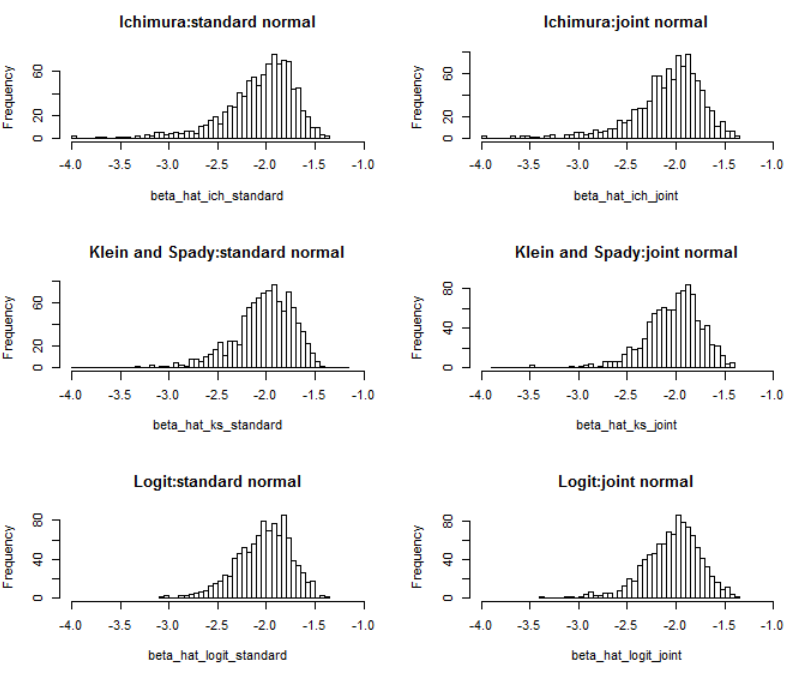
\includegraphics[width=\linewidth]{plot_comparison.png}
 
  \label{fig:plot of estimates}
\end{figure}

Combining simulation results from the table and the figure it can be observed that the distributions of all three estimators are skewed to the left, while the biases are bounded below $-0.06$. This indicates that the property of asymptotic consistency exists in all three estimators, amongst which the Klein and Spady's (1993) \cite{[12]} estimator converges most rapidly to the true value. 

As to what concerns the mean squared error, there is no significant difference among estimators in terms of magnitude. Since binary choice models are inherently heteroskedasticity, Ichimura’s (1993) \cite{[6]}  estimator would require the use of a weight function. However, this is out of the scope of our work and it is in fact also excluded from the np package. The weight function can be thus adapted to simulation in further studies. Nevertheless, our results suggest that this might not be an influencing issue here. 

In the end, a comparison between our simulation results and Hayfield and Racine's (2008) \cite{[28]} $NP\ Package$ encouraged us to rely on our original simulation functions. These results listed in the Appendix.

\section{Empirical Application} % (fold)
\label{sec:Empirical Application}

This section presents an empirical application on gender recognition by voice using the aforementioned statistical methods. A comparison with simple logistic regression is also made. 

The dataset we used is the pre-processed Gender Recognition by Voice and Speech Analysis dataset, a publicly available dataset from online resources containing 3,168 recorded voice samples by 1584 male and 1584 female speakers. 21 independent variables of acoustic properties of voice and 1 binary dependent indicator variable for gender are included in the dataset. More information regarding the dataset can be found in the appendix.  

As a first step, we removed three variables that have shown to cause multicollinearity problem,  namely; IQR, centroid, and dfrange. Next, the dataset is split into training sample for estimation of parameters, and test sample for prediction using estimated parameters. 70\% of the data are randomly selected into the training sample, with the remaining 30\% left for the test sample. 

For estimation, we use the pre-implemented np-package in R (Racine and Hayfield, 2008) \cite{[28]} for computational simplicity. In our self-implemented Ichimura (1993) method \cite{[6]} and Klein and Spady (1993) \cite{[12]} method, we employed grid-search in the minimization process for equation (9) and (14), which is also the method proposed by Ichimura (1993) \cite{[6]}. The minimization results are highly dependent on the specification of the grid for each independent variables and an appropriate resolution of the grid is necessary for precise results. As such, grid-search method suffers from the curse of dimensionality. Numerical approximation becomes infeasible in our case as the data contains 18 independent variables. We therefore decided to use the np-package which employs the $npksum()$ and $nlm()$ minimization procedures in R with multiple starting values to best avoid local minima. A comparison with logistic regression is also done using the logistic regression routine pre-implemented in R. 

The prediction results and the true values are plotted in figure 2. A comparison of in-sample and prediction accuracy rate and approximate calculation time are also presented in table 2. The accuracy rate is defined as ratio of correct gender prediction to the total number of data points.

\begin{table}
    \centering
	\begin{center}
	\begin{tabular}{  m{2cm} | m{3cm} c m{3cm} c m{3cm} |}
	  & Logistic Regression & Ichimura Method & Klein-Spady Method

	\tabularnewline
	\midrule

	Approximate calculation time & $<$ 1 second & $>$ 3 hours & $>$ 3 hours
	\tabularnewline
	\midrule

	In-sample Accuracy Rate (training sample) & 0.971145 & 0.974752 & 0.976104
	\tabularnewline
	\midrule

	Prediction Accuracy Rate (test sample) & 0.978947 &  0.977894 & 0.981052 
	\tabularnewline
	\bottomrule
	\end{tabular}
	\end{center}
	\caption {Estimation time and accuracy rate}
\end{table}

\bigskip
\bigbreak

\begin{figure}[H]

  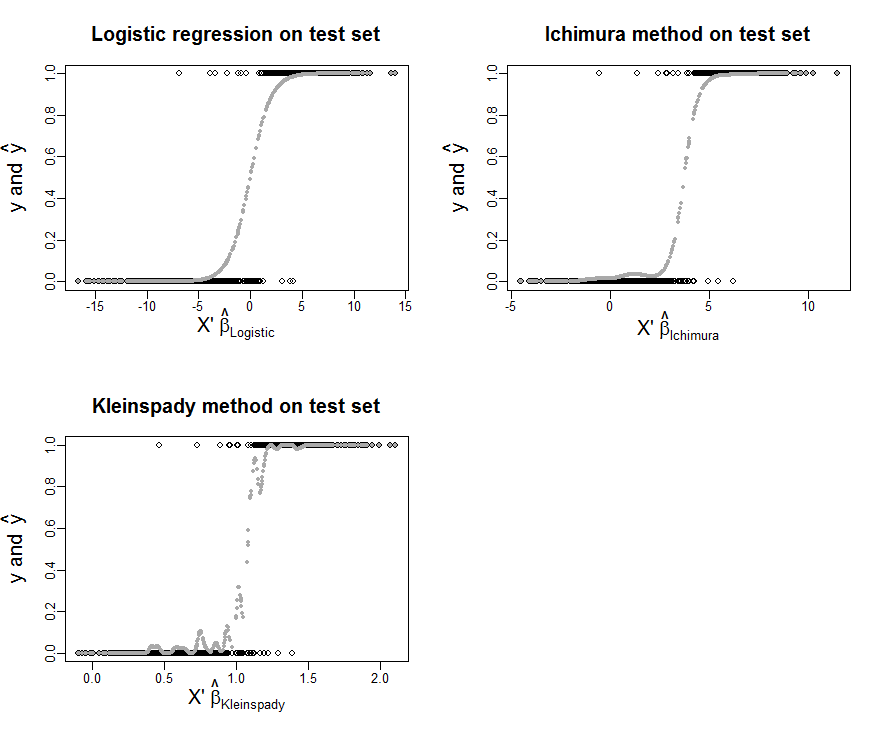
\includegraphics[width=\linewidth]{figure2.png}
 
  \label{fig: Plot of estimates on test sample}
  \caption{Plot of Estimates on Test Sample}
\end{figure}

From Table 2 and Figure 2, we could conclude that the logistic regression would be the preferred method in this case since the improvement in accuracy rate by using semi-parametric methods are minimum while the calculation time increases significantly. However, this could be due to the fact that the underlying data fit the logistic distribution better, and thus this comparison should not be generalized to other datasets. 

We also take note of the two peculiar features of the results. First, the accuracy rate is higher for test sample than in-sample accuracy rate. As the difference is relatively small, we postulate that this could be random and of no particular significance. Moreover, the fact that the training sample contains 3.5 times more data points than the test sample could exacerbate the random effect. The second feature is that the result graph from Klein and Spady (1993) \cite{[12]} method is not very smooth. This could be due to a problem with bandwidth selection included in the np-package (Racine and Hayfield, 2008) \cite{[28]} or the minimization process. However, as the result is not significantly worse than the other estimators, actually slightly better, we do not think that this should be of great concern.


\newpage 



\section{Bibliography} % (fold)
\label{sec:Bibliography}


\nocite{*}
\printbibliography[heading=none]

\newpage 

\section{Appendix}
\label{sec:appendix}

\subsection{List of Variables}
The following list shows the 21 independent variables and 1 binary gender indicator contained in the dataset.

\begin{center}
\begin{tabular}{ m{5em} | m{10cm}}
\toprule
Variable Name & Description
\tabularnewline
\midrule
meanfreq & mean frequency (in kHz)
\tabularnewline
sd & standard deviation of frequency
\tabularnewline
median & median frequency (in kHz)
\tabularnewline
Q25 & first quantile (in kHz)
\tabularnewline
Q75 & third quantile (in kHz)
\tabularnewline
IQR & interquartile range (in kHz)
\tabularnewline
skew & skewness
\tabularnewline
kurt & kurtosis
\tabularnewline
sp.ent & spectral antropy
\tabularnewline
sfm & spectral flatness
\tabularnewline
mode & mode frequency
\tabularnewline
centroid & frequency centroid
\tabularnewline
peakf & peak frequency (frequency with highest energy)
\tabularnewline
meanfun & average of fundamental frequency measured across acoustic signal
\tabularnewline
minfun & minimum fundamental frequency measured across acoustic signal
\tabularnewline
maxfun & maximum fundamental frequency measured across acoustic signal 
\tabularnewline
meandom & average of dominant frequency measured across acoustic signal 
\tabularnewline
mindom & minimum of dominant frequency measured across acoustic signal 
\tabularnewline
maxdom & maximum of dominant frequency measured across acoustic signal 
\tabularnewline
dfrange & range of dominant frequency measured across acoustic signal 
\tabularnewline
modindx & modulation index. Calculated as the accumulated absolute difference between adjacent measurements of fundamental frequencies divided by the frequency range 
\tabularnewline
label & male or female
\tabularnewline

\bottomrule
\end{tabular}
\end{center}


\subsection{Empirical Definition of Trimming Function}
Section 7 develops an empirical method to implement the trimming functions for Ichimura's (1993) \cite{[6]} and Klein and Spady's (1993) \cite{[12]} models.

Referring to theoretical definitions, the aim of a trimming function in Ichimura's (1993) \citep{[6]} model is to guarantee $\hat{p}_{-i}(X_i'\beta)$ is not too close to zero. 

The estimate $\hat{p}_{-i}(X_i'\beta)$ is calculated over a given bandwidth $h$. There are two ways to keep such an estimate far away enough from zero: either we  employ $A_\delta$  directly, which can be quite stringent, or we use observations that are close enough to the independent variables that satisfy $x \in A_\delta$. The latter also leads $\hat{p}_{-i}(X_i'\beta)$, the estimated probability for $X_i'\beta$, to be large enough. We use a similar reasoning to $A_n$ for the primary trimming function.

Before starting the estimation, simulated sample data is sieved by examining whether the single index's NW leave-one-out kernel estimates are large enough. A lower bound is defined, such that $\hat{p}(x'\beta)$ is not too close to zero and also so that enough observations are left  for the estimation to be reliable. If $\hat{p}(x'\beta)$ fails to achieve the chosen lower bound, this sample data $x$ will be removed from the data set.
Furthermore, as the Grid Search method is used to carry out the estimation, the same set of grids is used to define $\mathcal{B}$, as defined in section 4. Data sieving is carried out over this set such that the estimation procedure is sensible for each single grid.

Firstly, the same trimmed data set is used for Ichimura's (1993) \cite{[6]} and Klein and Spady's (1993) \cite{[12]} estimation methods. However, this is not enough for the latter model to work, as it only prevents $g(\cdot)$ from growing out of bounds.  Klein and Spady's (1993) \cite{[12]} model is more restrictive than Ichimura's (1993) \cite{[6]} model on this point, as it requires any estimate of $\hat{G}_i$ not to be too close to 0 or 1. Recall that the numerator follows the sum of dependent binary variables $y_i$ weighted by its corresponding kernel evaluation. This issue becomes apparent for relatively large evaluations. Therefore, we further introduce a lower bound equal to square root of machine double epsilon and set any estimate smaller than the lower bound to this value.


\subsection{A Comparison in Results of Simulation Functions and NP Package}
Model design of monte carlo simulation following Ichimura (1993):
\begin{itemize}
\item sample size is 250;
\item the semiparametric single index model is specified as binary choice model;
\item exogenous vector of variables contains two components and both are independently generated from standard normal distribution;
\item when constructing single index, parameter of the first exogenous component is normalized to 1, and true value for the second parameter is set to -2;
\item presume standard normal distribution for error distribution;
\item the amount of monte carlo simulation is 1000 times.
\end{itemize}
To summarize, the designed baseline function is
\begin{equation*}
y_i = I(x_{1i} - 2x_{2i} > \epsilon_i).
\end{equation*}

\begin{table}[H]
\caption {Mean Squared Error Comparison} \label{tab:mean squared error}

(with gridsearch $(-4, 0, 81)$)

\begin{tabular}{l r r}

\toprule
\textbf{method} & \textbf{NP Package} & \textbf{Simulation Functions} \tabularnewline\midrule
(standard normal distribution for $x_1$, $x_2$, $\epsilon$) & &
\tabularnewline
Ichimura & 0.00363 & 0.00201 \tabularnewline
Klein and Spady & 0.00416 & 0.0000893 \tabularnewline

\bottomrule
\end{tabular}
\end{table}

\begin{figure}[h!]
  \caption{Comparison of Estimates on the Same Scale}
  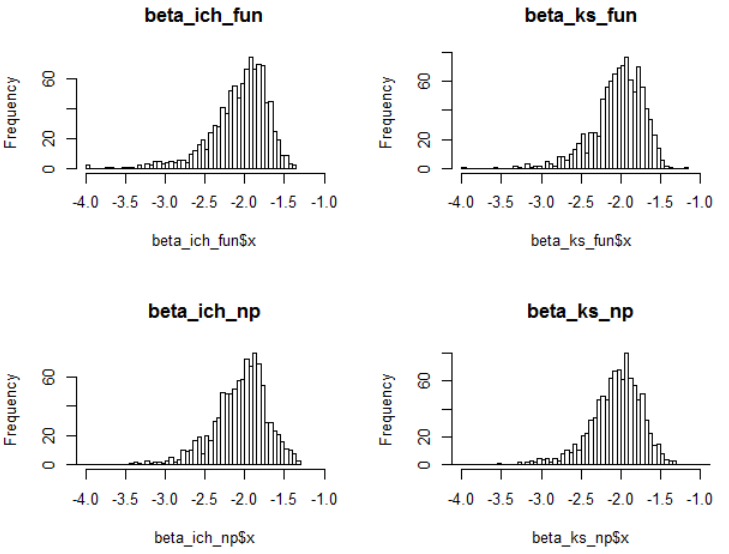
\includegraphics[width=\linewidth]{compare_done.png}
 
  \label{fig:comparison of estimates on the same scale}
\end{figure}

From $Table\ 3$ and $Figure\ 3$, we see that our self-implemented code does not perform significantly worse than the np-package. In fact it is even better for Klein and Spady's (1993) \cite{[12]} method. This could be due to the use of our \textit{a-priori} knowledge of the true beta when specifying the grid. We thus conclude that it is an useful and successful practice in constructing our own code for single index model functions.

\subsection{Optimization Methods: Grid Search $vs$ Non-linear Minimization}
\label{A comparison in optimization methods:grid search and non-linear squares}
We employed $Grid Search$ in the definition of simulation functions. Referring to $Figure\ 3$, this method is able to find `good' parameter values for a function. However a grid search has two deficiencies worth noticing: on the one hand, when either the size of the grid or the number of parameters to be estimated expands, the length of the first argument to grid search function (which is the support of estimates, i.e. $\mathcal{B}$ containing the true $\beta$) will increase, resulting in the number of necessary function evaluations growing exponentially; on the other hand, when the true $\beta$ is unknown, the performance of estimation relies heavily on the range of list and the distance between two candidates primarily set to loop over. In our simulation the support of $\mathcal{B}_2$ is presumably set to $(-4,0)$ with an accuracy rate of $0.05$. This leads to $81$ function evaluations for each data generation. Taking the amount of $1000$ data generations into account this method is already considerably computational costly even for estimation on a single parameter $\beta_2$. 

Hayfield and Racine's (2008)  \cite{[28]} np package employs a nonlinear parameter estimation tool ($optim: Nelder-Mead$) which does not require derivatives of objective functions and uses heuristics to search the domain of parameter. Compared to the support of $\mathcal{B}$ prespecified in Grid Search, the core function that facilitates this paper is $npindexbw$, which declares successful convergence in three ways: reaching absolute convergence tolerance, relative convergence tolerance or maximum number of iterations ($500$ times for Nelder-Mead method). Besides, this function provides a choice of different (random) initial points to start the searching, whereas in our simulation functions, starting points are manually chosen which may lead to ignorance of other local minima.

\end{document}
